\documentclass[conference]{IEEEtran}
\IEEEoverridecommandlockouts

\usepackage[T1]{fontenc}
\usepackage[utf8]{inputenc}
\usepackage{cite}
\usepackage{amsmath,amssymb,amsfonts}
\usepackage{graphicx}
\usepackage{booktabs}
\usepackage{array}
\usepackage{xcolor}
\usepackage{url}
\usepackage{tikz}
\usetikzlibrary{arrows.meta,positioning,shapes.geometric}
\usepackage[hidelinks]{hyperref}

\graphicspath{{figures/}}

% Traducción de etiquetas de IEEEtran (sin babel-spanish disponible)
\renewcommand{\abstractname}{Resumen}
\renewcommand{\IEEEkeywordsname}{Palabras clave}
\renewcommand{\refname}{Referencias}

\begin{document}

\title{Auditoría y Revalidación de un Sistema de Predicción de Diabetes
Basado en Aprendizaje Automático: Un Estudio de Caso sobre Fuga de
Información y Despliegue Clínico}

\author{\IEEEauthorblockN{Grupo de Investigación PREDIA}
\IEEEauthorblockA{\textit{Informática Clínica y Aprendizaje Automático Aplicado} \\
\textit{Proyecto PREDIA} \\
México \\
predia@example.org}}

\maketitle

\begin{abstract}
Los sistemas de aprendizaje automático se integran cada vez más en el software
clínico, pero su desempeño reportado suele aceptarse sin escrutinio
metodológico. Presentamos la auditoría del módulo de predicción de diabetes de
PREDIA, una plataforma de expediente clínico electrónico en producción cuyo
modelo anunciaba una exactitud del 97.89\%. Trabajando exclusivamente con los
propios artefactos del proyecto, mostramos que esa cifra no es reproducible ni
honesta: el estimador desplegado es una regresión logística codificada
directamente en TypeScript, entrenada sobre un conjunto distinto de 947 muestras
cuyas variables (urea, creatinina, VLDL) están ausentes del corpus de 100{,}000
filas de la plataforma, y su exactitud está inflada por \emph{fuga de
información} a través de la HbA1c, un criterio diagnóstico oficial de diabetes.
Una sonda validada por 5-fold confirma que la HbA1c por sí sola alcanza 0.93 de
ROC-AUC, mientras que un modelo de \emph{cribado} libre de fuga llega solo a
$\approx$0.66. Reentrenamos y comparamos nueve clasificadores bajo un protocolo
con control de fuga, validación cruzada estratificada y un panel de métricas de
orientación clínica; la regresión logística es el mejor modelo honesto (ROC-AUC
0.659, MCC 0.223). Lo interpretamos con importancia por permutación y SHAP, y lo
migramos a la API REST de PREDIA como un modelo TypeScript autocontenido con un
contrato de variables rediseñado y libre de fuga. El estudio aporta una
metodología de auditoría reproducible y un relato honesto de la brecha entre
métricas infladas y métricas honestas en el aprendizaje automático clínico.
\end{abstract}

\begin{IEEEkeywords}
fuga de información, predicción de diabetes, auditoría de modelos,
reproducibilidad, apoyo a la decisión clínica, interpretabilidad, aprendizaje
automático
\end{IEEEkeywords}

\section{Introducción}
La diabetes mellitus es una de las principales cargas de salud pública a nivel
mundial, afectando a unos 537 millones de adultos~\cite{idf2021atlas}. Dado que
la identificación temprana de individuos en riesgo permite intervenciones
preventivas, el aprendizaje automático (AA) se ha propuesto ampliamente para la
estratificación del riesgo de diabetes. Sin embargo, el valor clínico de tales
modelos depende por completo de la \emph{validez} de su desempeño reportado.
Cuando un modelo se evalúa incorrectamente---lo más común, mediante \emph{fuga
de información} (data leakage), el uso inadvertido de información no disponible
al momento de la predicción o que codifica el desenlace---las métricas
reportadas se inflan severamente y el sistema falla de forma silenciosa en
producción~\cite{kaufman2012leakage,kapoor2023leakage}.

Este artículo es un estudio de caso de exactamente ese tipo de fallo,
descubierto al auditar PREDIA, una plataforma de expediente clínico electrónico
(ECE) en producción. PREDIA distribuía un módulo de predicción de diabetes que
anunciaba una exactitud del 97.89\%. En lugar de aceptar esa cifra, sometimos el
modelo y sus datos a una auditoría reproducible usando únicamente los artefactos
del propio proyecto.

\textbf{Objetivos.} (i)~Determinar si la exactitud reportada por PREDIA es válida
y reproducible; (ii)~probar la existencia de fuga de información y fallos
metodológicos; (iii)~establecer una línea base honesta de desempeño reentrenando
y comparando múltiples clasificadores bajo un protocolo con control de fuga; y
(iv)~desplegar el modelo seleccionado de vuelta en PREDIA sin romper la
plataforma.

\textbf{Contribuciones.} (1)~Una auditoría formal y reproducible que demuestra
que la exactitud del modelo desplegado es a la vez irreproducible (entrenado en
un conjunto distinto con variables ausentes) e inflada por la fuga de la HbA1c.
(2)~Un \emph{benchmark} con control de fuga de nueve clasificadores, separando un
marco honesto de \emph{cribado} de un marco \emph{clínico} que cuantifica la
contribución de la fuga ($+0.285$ de ROC-AUC). (3)~Interpretabilidad y análisis
clínico del modelo honesto. (4)~Una migración a producción del modelo revalidado
hacia la API REST de PREDIA con un contrato de variables rediseñado y libre de
fuga.

\section{Trabajos Relacionados}
Los aprendices basados en árboles y en kernels dominan la predicción clínica
tabular: bosques aleatorios~\cite{breiman2001random}, árboles potenciados por
gradiente como los de XGBoost~\cite{chen2016xgboost} y
LightGBM~\cite{ke2017lightgbm}, máquinas de soporte
vectorial~\cite{cortes1995svm} y clasificadores por vecinos más
cercanos~\cite{cover1967knn}. Todos los experimentos aquí emplean el ecosistema
\texttt{scikit-learn}~\cite{pedregosa2011scikit}. Para la interpretabilidad del
modelo adoptamos los valores SHAP~\cite{lundberg2017shap} junto con la
importancia por permutación~\cite{breiman2001random}.

La fuga de información es una amenaza reconocida desde hace tiempo pero
persistente para la validez de los estudios de AA~\cite{kaufman2012leakage};
trabajos recientes la documentan como un motor primario de la crisis de
reproducibilidad en la ciencia basada en AA en múltiples
disciplinas~\cite{kapoor2023leakage}. En contextos clínicos, la fuga surge con
frecuencia al incluir mediciones diagnósticas que \emph{definen} la etiqueta. El
diagnóstico de diabetes se rige por umbrales de laboratorio---siendo la HbA1c
$\geq 6.5\%$ un criterio primario~\cite{ada2021classification}---de modo que
cualquier modelo que consuma HbA1c para predecir una etiqueta derivada de la
HbA1c está, por construcción, filtrando información. Como la exactitud es
engañosa bajo desbalance de clases, reportamos el coeficiente de correlación de
Matthews (MCC), más informativo para la clasificación
binaria~\cite{chicco2020mcc}. Finalmente, el modelo original de PREDIA fue
entrenado sobre un pequeño conjunto público de diabetes~\cite{rashid2020diabetes}
cuyo conjunto de variables difiere de los datos operativos de la
plataforma---una discrepancia central en nuestros hallazgos.

\section{Metodología}
\subsection{Conjunto de datos}
Todos los experimentos usan \texttt{diabetes\_dataset.csv}, el corpus
distribuido con el repositorio de PREDIA (Tabla~\ref{tab:dataset}). Contiene
100{,}000 instancias y 31 atributos que describen demografía, situación
socioeconómica, estilo de vida, antropometría, signos vitales, perfil lipídico y
mediciones de laboratorio. El objetivo binario \texttt{diagnosed\_diabetes}
presenta un desbalance leve (60.0\% positivo / 40.0\% negativo, razón 1.50). El
corpus no tiene valores faltantes ni filas duplicadas.

\begin{table}[!t]
\renewcommand{\arraystretch}{1.2}
\caption{Características del corpus \texttt{diabetes\_dataset.csv}}
\label{tab:dataset}
\centering
\begin{tabular}{l l}
\toprule
\textbf{Propiedad} & \textbf{Valor} \\
\midrule
Instancias & 100{,}000 \\
Columnas totales & 31 \\
Atributos numéricos & 24 (incl.\ objetivo) \\
Atributos categóricos & 7 \\
Variable objetivo & \texttt{diagnosed\_diabetes} \\
Clase positiva (Diabetes) & 59{,}998 (60.0\%) \\
Clase negativa (No Diabetes) & 40{,}002 (40.0\%) \\
Razón de desbalance & 1.50 \\
Valores faltantes & 0 \\
Filas duplicadas & 0 \\
Partición train/test & 80{,}000 / 20{,}000 (estratificada) \\
\bottomrule
\end{tabular}
\end{table}


\subsection{Taxonomía de variables con control de fuga}
La decisión metodológica definitoria de este estudio es una taxonomía explícita
de variables que controla la fuga:
\begin{itemize}
\item \textbf{Fuga directa (siempre eliminadas):} \texttt{diabetes\_stage} (la
categoría diagnóstica en sí) y \texttt{diabetes\_risk\_score} (un proxy de
riesgo derivado).
\item \textbf{Laboratorios diagnósticos:} \texttt{hba1c},
\texttt{glucose\_fasting}, \texttt{glucose\_postprandial} e
\texttt{insulin\_level}. Por ser criterios diagnósticos, se \emph{excluyen} del
marco honesto de \emph{cribado} y se \emph{incluyen} solo en un marco
\emph{clínico} usado para cuantificar su contribución (con fuga).
\item \textbf{Variables de cribado:} demografía, situación socioeconómica,
estilo de vida, antecedentes familiares, antropometría, signos vitales y perfil
lipídico---las 24 entradas que una herramienta de riesgo pre-diagnóstica puede
recolectar legítimamente.
\end{itemize}
La Fig.~\ref{fig:leakcorr} confirma que las variables más correlacionadas con el
objetivo son precisamente los laboratorios diagnósticos, lo que motiva esta
separación.

\begin{figure}[!t]
\centering
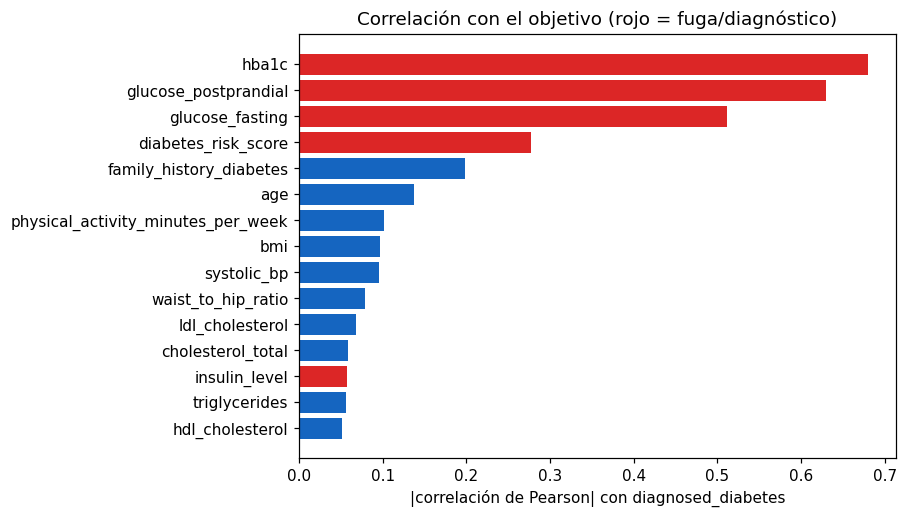
\includegraphics[width=\columnwidth]{leakage_correlation.png}
\caption{Correlación de Pearson absoluta con el objetivo. Las señales más fuertes
(rojo) son variables diagnósticas/con fuga (\texttt{hba1c}, \texttt{glucose\_*},
\texttt{diabetes\_risk\_score}); las variables legítimas de cribado (azul) están
débilmente correlacionadas.}
\label{fig:leakcorr}
\end{figure}

\subsection{Preprocesamiento, validación y pipeline}
Los atributos categóricos se codifican con one-hot y los numéricos se
estandarizan ($z$-score); los binarios se mantienen. Todas las transformaciones
se ajustan \emph{dentro} de un \texttt{Pipeline} de
\texttt{scikit-learn}~\cite{pedregosa2011scikit} para evitar la contaminación
train/test. Usamos una partición estratificada 80/20 y validación cruzada
estratificada de 4 particiones para la selección de modelos, con una semilla
global de 42 para reproducibilidad total. La Fig.~\ref{fig:pipeline} resume el
protocolo de extremo a extremo.

\begin{figure}[!t]
\centering
\resizebox{0.95\columnwidth}{!}{%
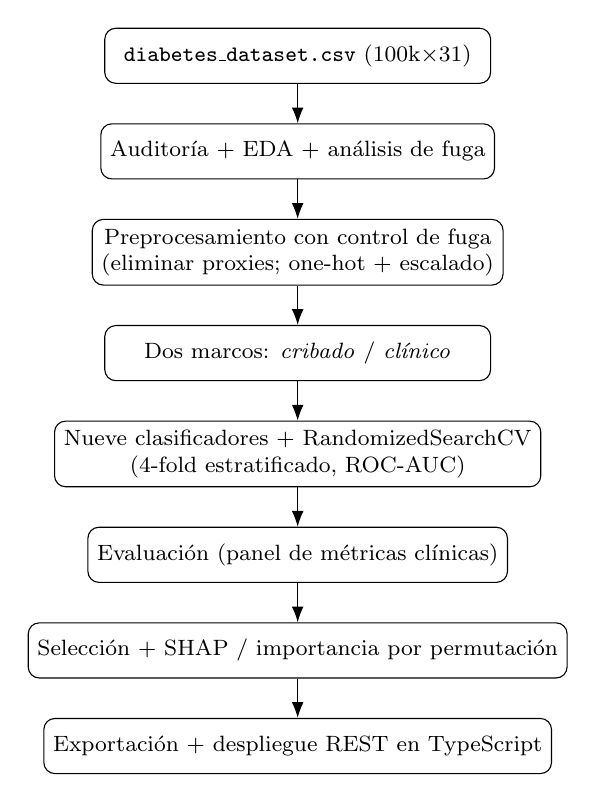
\begin{tikzpicture}[
  node distance=5mm,
  box/.style={draw, rounded corners, align=center, font=\footnotesize,
              minimum width=4.9cm, minimum height=7mm},
  arr/.style={-{Latex[length=2mm]}}]
\node[box] (data) {\texttt{diabetes\_dataset.csv} (100k$\times$31)};
\node[box, below=of data] (audit) {Auditoría + EDA + análisis de fuga};
\node[box, below=of audit] (prep) {Preprocesamiento con control de fuga\\(eliminar proxies; one-hot + escalado)};
\node[box, below=of prep] (fram) {Dos marcos: \emph{cribado} / \emph{clínico}};
\node[box, below=of fram] (zoo) {Nueve clasificadores + RandomizedSearchCV\\(4-fold estratificado, ROC-AUC)};
\node[box, below=of zoo] (eval) {Evaluación (panel de métricas clínicas)};
\node[box, below=of eval] (sel) {Selección + SHAP / importancia por permutación};
\node[box, below=of sel] (dep) {Exportación + despliegue REST en TypeScript};
\foreach \a/\b in {data/audit,audit/prep,prep/fram,fram/zoo,zoo/eval,eval/sel,sel/dep}
  \draw[arr] (\a) -- (\b);
\end{tikzpicture}}
\caption{Pipeline reproducible de auditoría a despliegue.}
\label{fig:pipeline}
\end{figure}

\section{Auditoría del Modelo Original}
\subsection{Arquitectura y desempeño reportado}
La inspección del artefacto serializado (\texttt{modelo\_diabetes.pkl}) muestra
que el estimador desplegado es una \emph{regresión logística} con 11 variables
de entrada (\texttt{Gender, AGE, Urea, Cr, HbA1c, Chol, TG, HDL, LDL, VLDL,
BMI}), un único intercepto de $7.578$, entrenada con 947 muestras (757 train /
190 test). Los metadatos de la plataforma y la semilla de la base de datos
reportan una exactitud de $0.9789$, mientras que la documentación en el código
afirma simultáneamente $98.42\%$ de exactitud, $100\%$ de precisión y $0.9975$ de
AUC---una inconsistencia interna que ya socava la confianza.

\subsection{Reproducibilidad y discrepancia de datos/variables}
No existe código de entrenamiento ni notebook en el repositorio; la metodología,
por tanto, no es reproducible. Además, el modelo desplegado fue entrenado sobre
un corpus distinto (el conjunto público de 947 muestras~\cite{rashid2020diabetes}):
tres de sus once variables---\texttt{Urea}, \texttt{Cr} y \texttt{VLDL}---están
\emph{ausentes} del conjunto operativo de PREDIA, y las variables lipídicas usan
una escala de unidades incompatible. El modelo no puede evaluarse tal cual sobre
los propios datos de la plataforma. Observamos además que, en tiempo de
servicio, el modelo no se carga desde el archivo \texttt{.pkl}, sino que se
reimplementa como coeficientes codificados directamente en TypeScript,
aumentados con reglas clínicas escritas a mano.

\subsection{Fuga de información}
La HbA1c es la segunda variable más importante del modelo original, pero HbA1c
$\geq 6.5\%$ \emph{es} el criterio diagnóstico de diabetes~\cite{ada2021classification}.
Usarla como predictor, por tanto, filtra la etiqueta. La Tabla~\ref{tab:leakage}
cuantifica esto con regresiones logísticas validadas por 5-fold sobre
subconjuntos aislados de variables: la HbA1c por sí sola ya produce 0.93 de
ROC-AUC, el par de puros proxies \texttt{diabetes\_stage}+\texttt{risk\_score}
alcanza 0.997, mientras que un subconjunto de cribado libre de fuga llega solo a
0.61. La exactitud reportada de $\approx$98\% es, así, solo alcanzable con
variables diagnósticas/con fuga; refleja fuga, no capacidad predictiva
pre-diagnóstica.

\begin{table}[!t]
\renewcommand{\arraystretch}{1.2}
\caption{Demostración de fuga: regresión logística validada por 5-fold
entrenada sobre subconjuntos aislados de variables de
\texttt{diabetes\_dataset.csv}}
\label{tab:leakage}
\centering
\begin{tabular}{l c c}
\toprule
\textbf{Subconjunto de variables} & \textbf{Exactitud} & \textbf{ROC-AUC} \\
\midrule
\texttt{hba1c} solamente & 0.8520 & 0.9325 \\
\texttt{glucose\_fasting} solamente & 0.7307 & 0.8082 \\
Labs.\ diagnósticos (HbA1c+glucosa+insulina) & 0.8567 & 0.9337 \\
\texttt{diabetes\_stage}+\texttt{risk\_score} & \textbf{0.9979} & \textbf{0.9974} \\
\midrule
Cribado (numéricas no diagnósticas) & 0.6163 & 0.6121 \\
\bottomrule
\end{tabular}
\end{table}


\section{Experimentación}
Reentrenamos nueve clasificadores bajo el marco de cribado: regresión logística,
bosque aleatorio~\cite{breiman2001random}, extra trees, gradient boosting por
histograma, XGBoost~\cite{chen2016xgboost}, LightGBM~\cite{ke2017lightgbm},
máquina de soporte vectorial (kernel RBF)~\cite{cortes1995svm}, $k$ vecinos más
cercanos~\cite{cover1967knn} y un perceptrón multicapa. Cada estimador se
envuelve en el pipeline común de preprocesamiento y se ajusta con
\texttt{RandomizedSearchCV} (8 candidatos, 4-fold estratificado, métrica
ROC-AUC). Dado que el SVM con kernel y el KNN escalan mal a $8\times10^4$ filas
de entrenamiento, se ajustan sobre una submuestra estratificada de 8{,}000 filas
y se evalúan sobre el conjunto de test completo; esto se reporta explícitamente.
Todas las ejecuciones comparten \texttt{random\_state}=42.

\section{Resultados}
La Tabla~\ref{tab:comparison} reporta el desempeño en test de los nueve modelos
bajo el marco honesto de cribado. Destacan tres hallazgos. Primero, el problema
honesto es genuinamente difícil: todos los modelos se agrupan alrededor de
ROC-AUC $0.65$--$0.66$. Segundo, \emph{la regresión logística es el mejor modelo
honesto} por ROC-AUC ($0.6591$) y por MCC ($0.2229$), y es también el mejor
calibrado y más equilibrado. Tercero, los ensambles de árboles y el SVM cambian
especificidad por sensibilidad (p.\ ej.\ el SVM alcanza $0.96$ de sensibilidad
pero $0.09$ de especificidad), lo que infla la F1 sin mejorar la discriminación.
Los resúmenes comparativos de ROC y ROC-AUC se muestran en las
Figs.~\ref{fig:roc} y~\ref{fig:auc}; la matriz de confusión y el diagrama de
fiabilidad del modelo seleccionado aparecen en las Figs.~\ref{fig:cm}
y~\ref{fig:cal}.

\input{tables/comparison_es}

\begin{figure}[!t]
\centering
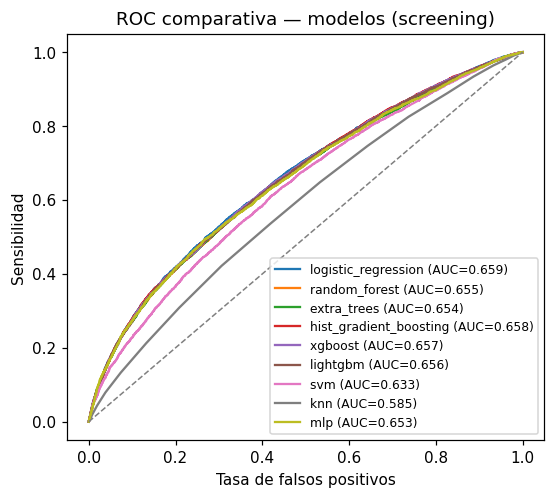
\includegraphics[width=\columnwidth]{comparison_roc.png}
\caption{Curvas ROC comparativas de los nueve clasificadores (marco de cribado).}
\label{fig:roc}
\end{figure}

\begin{figure}[!t]
\centering
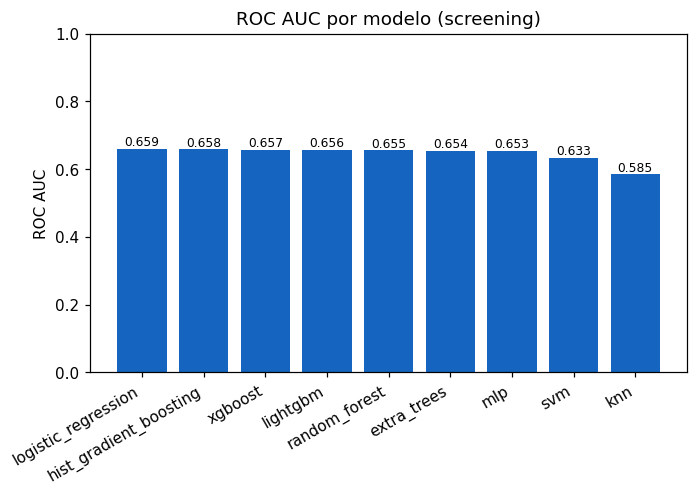
\includegraphics[width=\columnwidth]{comparison_auc.png}
\caption{ROC-AUC por modelo (marco de cribado).}
\label{fig:auc}
\end{figure}

\begin{figure}[!t]
\centering
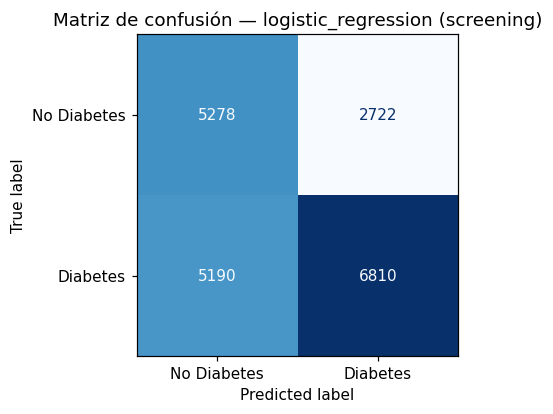
\includegraphics[width=0.78\columnwidth]{cm_screening_logistic_regression.png}
\caption{Matriz de confusión del modelo de cribado de regresión logística
seleccionado sobre el conjunto de test de 20{,}000 instancias.}
\label{fig:cm}
\end{figure}

\begin{figure}[!t]
\centering
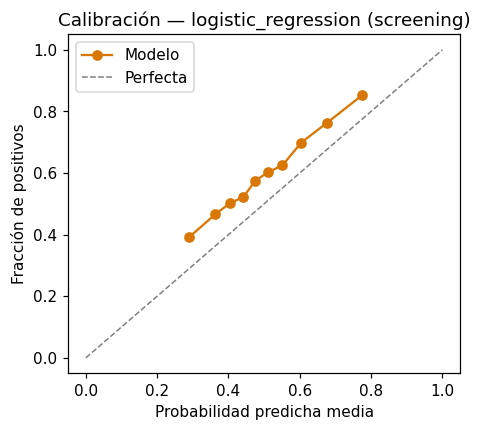
\includegraphics[width=0.82\columnwidth]{cal_screening_logistic_regression.png}
\caption{Diagrama de fiabilidad (calibración) del modelo seleccionado.}
\label{fig:cal}
\end{figure}

Para cuantificar la contribución de la fuga de forma directa, la
Tabla~\ref{tab:framing} contrasta el marco de cribado con un marco clínico que
reintroduce los laboratorios diagnósticos. Añadir esas variables eleva la
ROC-AUC de $\approx$0.66 a $\approx$0.94---un aumento medio de $+0.285$---lo que
confirma que la aparente excelencia del sistema original era casi enteramente
fuga.

\begin{table}[!t]
\renewcommand{\arraystretch}{1.2}
\caption{Efecto de incluir variables de laboratorio diagnósticas: marco honesto
de \emph{cribado} vs.\ marco \emph{clínico} (con HbA1c, glucosa e insulina). La
brecha de ROC-AUC cuantifica la contribución de la fuga de información.}
\label{tab:framing}
\centering
\begin{tabular}{l c c c c}
\toprule
& \multicolumn{2}{c}{\textbf{Cribado}} & \multicolumn{2}{c}{\textbf{Clínico}} \\
\cmidrule(lr){2-3}\cmidrule(lr){4-5}
\textbf{Modelo} & Exa. & ROC-AUC & Exa. & ROC-AUC \\
\midrule
Regresión Logística & 0.6044 & 0.6591 & 0.8878 & 0.9339 \\
Random Forest       & 0.6244 & 0.6549 & 0.9196 & 0.9417 \\
XGBoost             & 0.6289 & 0.6573 & 0.9199 & 0.9444 \\
\midrule
\multicolumn{1}{l}{\textbf{Media $\Delta$ ROC-AUC}} & \multicolumn{4}{c}{$+0.285$ (contribución de la fuga)} \\
\bottomrule
\end{tabular}
\end{table}


\section{Interpretabilidad}
Interpretamos el modelo seleccionado con importancia por permutación (caída en la
ROC-AUC de test) y valores SHAP~\cite{lundberg2017shap}. Ambos métodos coinciden
de cerca (Tabla~\ref{tab:importance}, Figs.~\ref{fig:perm} y~\ref{fig:shap}):
\texttt{family\_history\_diabetes}, \texttt{age} y
\texttt{physical\_activity\_minutes\_per\_week} dominan, seguidas de \texttt{bmi}
y \texttt{diet\_score}.

\begin{table}[!t]
\renewcommand{\arraystretch}{1.2}
\caption{Variables más influyentes del modelo de cribado seleccionado, por
importancia de permutación (caída en ROC-AUC) y por valor SHAP absoluto medio.}
\label{tab:importance}
\centering
\begin{tabular}{l c | l c}
\toprule
\multicolumn{2}{c|}{\textbf{Importancia por permutación}} & \multicolumn{2}{c}{\textbf{SHAP (\(|\phi|\) medio)}} \\
Variable & $\Delta$AUC & Variable & $|\phi|$ \\
\midrule
family\_history\_diabetes & 0.0816 & age & 0.0539 \\
age & 0.0340 & family\_history\_diabetes & 0.0536 \\
physical\_activity & 0.0179 & physical\_activity & 0.0362 \\
bmi & 0.0037 & bmi & 0.0220 \\
diet\_score & 0.0023 & diet\_score & 0.0126 \\
hdl\_cholesterol & 0.0013 & hdl\_cholesterol & 0.0125 \\
screen\_time & 0.0012 & triglycerides & 0.0082 \\
triglycerides & 0.0008 & screen\_time & 0.0076 \\
\bottomrule
\end{tabular}
\end{table}


\begin{figure}[!t]
\centering

\includegraphics[width=\columnwidth]{permutation_importance.png}
\caption{Importancia por permutación del modelo de cribado seleccionado.}
\label{fig:perm}
\end{figure}

\begin{figure}[!t]
\centering
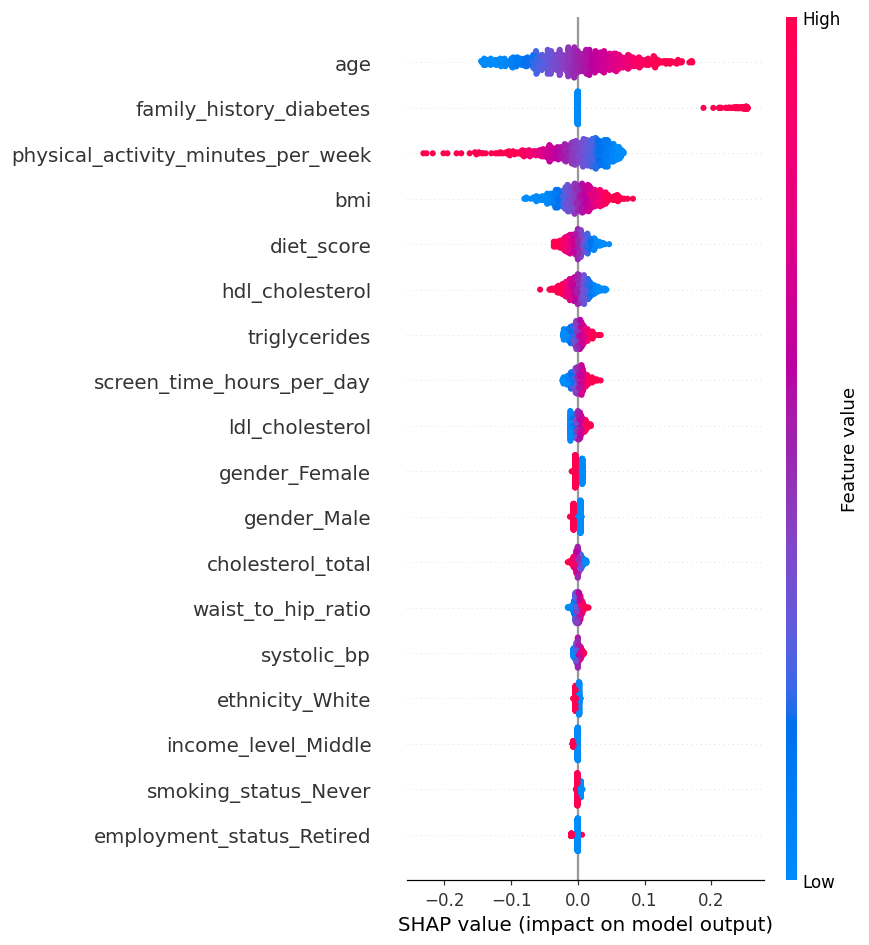
\includegraphics[width=\columnwidth]{shap_summary.png}
\caption{Resumen SHAP (beeswarm) del modelo de cribado seleccionado.}
\label{fig:shap}
\end{figure}

\textbf{Impacto clínico.} De forma tranquilizadora, los predictores dominantes
son \emph{modificables o registrables de forma rutinaria} sin pruebas de
laboratorio (antecedentes familiares, actividad física, índice de masa corporal,
dieta), que es exactamente en lo que una herramienta de cribado pre-diagnóstico
debería apoyarse. \textbf{Riesgos de interpretación.} La importancia no implica
causalidad; las asociaciones son observacionales, el corpus es de procedencia
desconocida y los tamaños de efecto modestos implican que las predicciones
individuales conllevan una incertidumbre sustancial.

\section{Discusión}
\textbf{Por qué el modelo original parecía excelente.} Su exactitud de
$\approx$98\% fue el producto conjunto de dos artefactos: la evaluación sobre un
conjunto de datos distinto y más pequeño, y la fuga de información a través de la
HbA1c. Ninguno refleja la capacidad del modelo para anticipar la diabetes antes
del diagnóstico.
\textbf{Métricas infladas vs.\ honestas.} El mismo algoritmo (regresión
logística) pasa de ROC-AUC $0.93$ (con fuga) a $0.66$ (libre de fuga); la
exactitud bajo desbalance es especialmente engañosa aquí, razón por la cual
enfatizamos el MCC y la exactitud balanceada~\cite{chicco2020mcc}.
\textbf{Implicaciones clínicas.} Una señal pre-diagnóstica honesta de ROC-AUC
$\approx$0.66 es modesta; el modelo solo es defendible como \emph{apoyo} a la
decisión y nunca debe presentarse como un diagnóstico.
\textbf{Limitaciones del conjunto de datos.} El corpus tiene apariencia
sintética, procedencia no documentada, carece de validez externa y agrupa
variables que definen el diagnóstico, lo que vuelve peligroso el modelado
ingenuo.
\textbf{Riesgos de despliegue.} Distribuir un modelo inflado por fuga invita al
sesgo de automatización y a una confianza clínica insegura; esto motivó tanto la
revalidación como el contrato de variables rediseñado.

\section{Integración en Producción}
El modelo revalidado se integró en PREDIA preservando las restricciones de la
plataforma. (i)~\textbf{Decisión de arquitectura:} el runtime de servicio es
TypeScript puro (sin proceso auxiliar de Python), elegido por portabilidad; por
ello exportamos el modelo de cribado de regresión logística---que es además el
mejor modelo honesto---como coeficientes simples más los parámetros de
one-hot/escalado, consumidos genéricamente en inferencia. (ii)~\textbf{
Exportación:} el pipeline completo de \texttt{scikit-learn} se serializa
(\texttt{joblib}/\texttt{pickle}) para reproducibilidad, y se genera un archivo
JSON de parámetros para el runtime de TypeScript. (iii)~\textbf{API REST:} el
endpoint \texttt{/api/predicciones/nueva} y su esquema de validación se migraron
al nuevo contrato de 24 variables libre de fuga; el formulario web de predicción
se reescribió en consecuencia. (iv)~\textbf{Compatibilidad:} las \emph{lecturas}
de predicciones (p.\ ej.\ la aplicación móvil) no se vieron afectadas, ya que
solo cambió la \emph{creación} de predicciones; los metadatos del modelo se
corrigieron del inflado 97.89\% al valor honesto. Una prueba de extremo a
extremo confirmó que el endpoint migrado devuelve predicciones coherentes.

\section{Conclusiones}
Auditamos un sistema de predicción de diabetes en producción y mostramos, usando
únicamente la evidencia del propio proyecto, que su exactitud insignia del
97.89\% no era reproducible ni honesta: provenía de una discrepancia de
datos/variables y de fuga de información mediada por la HbA1c. Un nuevo
\emph{benchmark} con control de fuga de nueve modelos estableció una línea base
honesta (regresión logística, ROC-AUC $0.659$, MCC $0.223$), que interpretamos y
redesplegamos en PREDIA con un contrato de variables corregido. La lección
central es metodológica: en el AA clínico, las métricas casi perfectas son una
señal de alarma, y el control disciplinado de la fuga, la reproducibilidad y el
reporte honesto importan más que la exactitud insignia.

\section{Trabajo Futuro}
Las direcciones futuras incluyen: recolectar una cohorte más grande, etiquetada
clínicamente y documentada; validación externa multicéntrica y temporal;
calibración de probabilidades y optimización del umbral según el costo clínico
(favoreciendo la sensibilidad); análisis de equidad por subgrupos de etnia y
sexo; \emph{aprendizaje federado} con preservación de la privacidad entre
instituciones; y herramientas más ricas de IA explicable integradas en el flujo
de trabajo del clínico.

\section*{Reproducibilidad}
Todos los artefactos (notebooks ejecutados, modelos entrenados, métricas,
figuras e informes) se proporcionan en el directorio \texttt{ml-research/} con un
\texttt{requirements.txt} de versiones fijadas y una semilla global de 42.

\bibliographystyle{IEEEtran}
\bibliography{references}

\end{document}
